\begin{minipage}{0.75\linewidth}
\begin{figure}[h]
    \centering
    \begin{adjustbox}{max width=1.0\linewidth, keepaspectratio}
        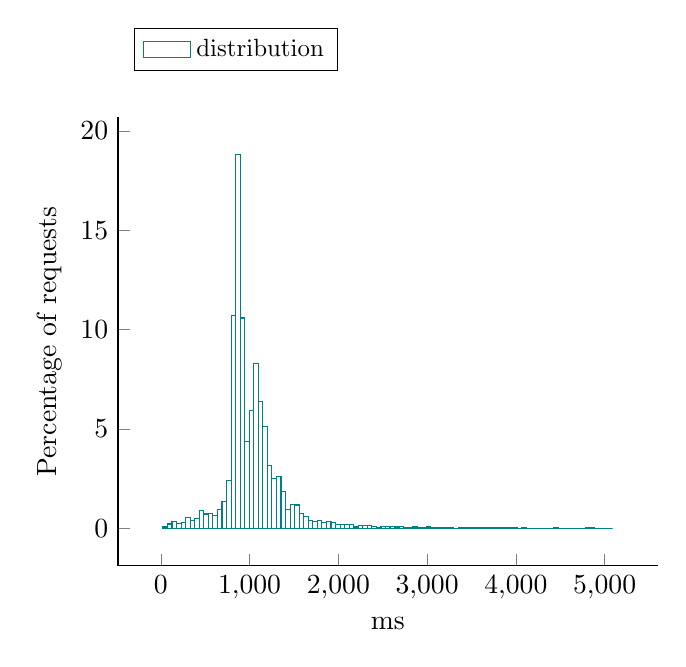
\begin{tikzpicture}
            \begin{axis}[ylabel = Percentage of requests, 
xlabel = ms, 
legend style = {nodes={scale=0.9, transform shape}, at={(0.03,1.2)}, anchor=north west, draw=black, fill=white, align=left, legend columns=3},
area style, mark size = 0pt,
 cycle list name = exotic,
  axis lines* = left]
		\addplot +[ybar interval] coordinates {
			 (24, 0.0625)
			 (75.17, 0.21875)
			 (126.34, 0.34375)
			 (177.51, 0.25)
			 (228.68, 0.28125)
			 (279.85, 0.5625)
			 (331.02, 0.390625)
			 (382.19, 0.5)
			 (433.36, 0.90625)
			 (484.53, 0.71875)
			 (535.7, 0.75)
			 (586.87, 0.625)
			 (638.04, 0.953125)
			 (689.21, 1.34375)
			 (740.38, 2.40625)
			 (791.55, 10.7188)
			 (842.72, 18.7969)
			 (893.89, 10.5781)
			 (945.06, 4.35938)
			 (996.23, 5.9375)
			 (1047.4, 8.29688)
			 (1098.57, 6.39062)
			 (1149.74, 5.14062)
			 (1200.91, 3.15625)
			 (1252.08, 2.5)
			 (1303.25, 2.59375)
			 (1354.42, 1.85938)
			 (1405.59, 0.9375)
			 (1456.76, 1.21875)
			 (1507.93, 1.17188)
			 (1559.1, 0.765625)
			 (1610.27, 0.578125)
			 (1661.44, 0.40625)
			 (1712.61, 0.359375)
			 (1763.78, 0.390625)
			 (1814.95, 0.3125)
			 (1866.12, 0.328125)
			 (1917.29, 0.3125)
			 (1968.46, 0.171875)
			 (2019.63, 0.171875)
			 (2070.8, 0.1875)
			 (2121.97, 0.203125)
			 (2173.14, 0.0625)
			 (2224.31, 0.125)
			 (2275.48, 0.125)
			 (2326.65, 0.140625)
			 (2377.82, 0.09375)
			 (2428.99, 0.046875)
			 (2480.16, 0.109375)
			 (2531.33, 0.09375)
			 (2582.5, 0.078125)
			 (2633.67, 0.0625)
			 (2684.84, 0.09375)
			 (2736.01, 0.03125)
			 (2787.18, 0.015625)
			 (2838.35, 0.0625)
			 (2889.52, 0.03125)
			 (2940.69, 0.046875)
			 (2991.86, 0.0625)
			 (3043.03, 0.03125)
			 (3094.2, 0.03125)
			 (3145.37, 0.046875)
			 (3196.54, 0.03125)
			 (3247.71, 0.03125)
			 (3298.88, 0)
			 (3350.05, 0.015625)
			 (3401.22, 0.015625)
			 (3452.39, 0.03125)
			 (3503.56, 0.03125)
			 (3554.73, 0.03125)
			 (3605.9, 0.046875)
			 (3657.07, 0.015625)
			 (3708.24, 0.046875)
			 (3759.41, 0.015625)
			 (3810.58, 0.015625)
			 (3861.75, 0.015625)
			 (3912.92, 0.015625)
			 (3964.09, 0.015625)
			 (4015.26, 0)
			 (4066.43, 0.015625)
			 (4117.6, 0)
			 (4168.77, 0)
			 (4219.94, 0)
			 (4271.11, 0)
			 (4322.28, 0)
			 (4373.45, 0)
			 (4424.62, 0.015625)
			 (4475.79, 0)
			 (4526.96, 0)
			 (4578.13, 0)
			 (4629.3, 0)
			 (4680.47, 0)
			 (4731.64, 0)
			 (4782.81, 0.015625)
			 (4833.98, 0.015625)
			 (4885.15, 0)
			 (4936.32, 0)
			 (4987.49, 0)
			 (5038.66, 0)
			 (5089.83, 0)
		};
\addlegendentry{distribution};
           \end{axis}
      \end{tikzpicture}
  \end{adjustbox}
  \caption{Response time distribution - req = ReadTimeline-0}
\end{figure}
\end{minipage}\hfill\begin{minipage}{0.18\linewidth}
\begin{table}[h]
\begin{tabular}{|cc|}
\hline
\textbf{} & \textbf{ms}\\ \hline
 \Xhline{0.005\arrayrulewidth}
min & 24\\
 \Xhline{0.005\arrayrulewidth}
max & 5141\\
 \Xhline{0.005\arrayrulewidth}
mean & 1037\\
 \Xhline{0.005\arrayrulewidth}
std & 386\\
\hline
\hline
 \Xhline{0.005\arrayrulewidth}
25th & 853\\
 \Xhline{0.005\arrayrulewidth}
50th & 942\\
 \Xhline{0.005\arrayrulewidth}
75th & 1145\\
 \Xhline{0.005\arrayrulewidth}
80th & 1195\\
 \Xhline{0.005\arrayrulewidth}
85th & 1277\\
 \Xhline{0.005\arrayrulewidth}
90th & 1391\\
 \Xhline{0.005\arrayrulewidth}
95th & 1636\\
 \Xhline{0.005\arrayrulewidth}
99th & 2622\\
\hline
\end{tabular}
\caption{Response time}
\end{table}
\end{minipage}\hfill